%tikz_draw
\documentclass[11pt,a4paper]{article}
\usepackage[utf8]{inputenc}
\usepackage[english]{babel}
\usepackage{amsmath}
\usepackage{amsfonts}
\usepackage{amssymb}
\usepackage[left=2cm,right=2cm,top=2cm,bottom=2cm]{geometry}
\usepackage{tikz}
%preamble

\begin{document}

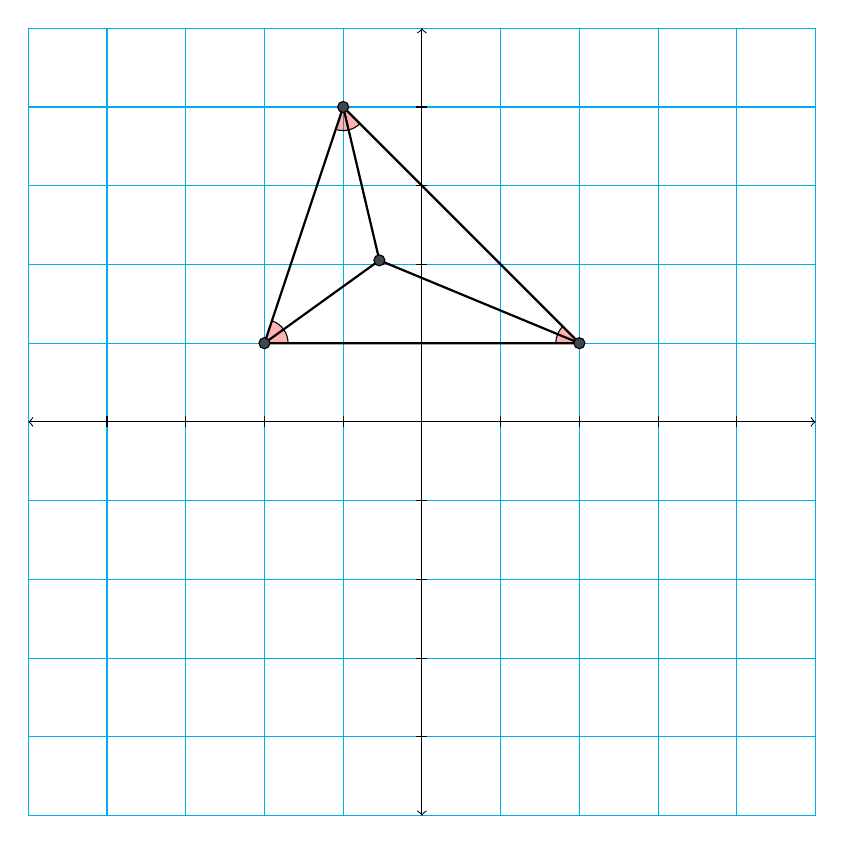
\begin{tikzpicture}

\draw[cyan] (-5, 5) grid (5, -5);

    %axis
    \draw[<->] (-5,0) -- (5,0);
    \draw[<->] (0, -5) -- (0, 5);

    %axis ticks
    \foreach \x in {-4,-3,...,3,4}
        \draw (\x,-2pt) -- (\x,2pt);
%

    \foreach \x in {-4,-3,...,3,4}
        \draw (-2pt,\x) -- (2pt,\x);

\fill[red, opacity=0.3] (-2, 1) -- ([shift=(0.0:0.3)]-2,1) arc[start angle=0.0, end angle=71.56505117707799, radius=0.3] -- cycle;
\draw  ([shift=(0.0:0.3)]-2,1) arc[start angle=0.0, end angle=71.56505117707799, radius=0.3];
\fill[red, opacity=0.3] (-1, 4) -- ([shift=(-45.0:0.3)]-1,4) arc[start angle=-45.0, end angle=-108.43494882292202, radius=0.3] -- cycle;
\draw  ([shift=(-45.0:0.3)]-1,4) arc[start angle=-45.0, end angle=-108.43494882292202, radius=0.3];
\fill[red, opacity=0.3] (2, 1) -- ([shift=(135.0:0.3)]2,1) arc[start angle=135.0, end angle=180.0, radius=0.3] -- cycle;
\draw  ([shift=(135.0:0.3)]2,1) arc[start angle=135.0, end angle=180.0, radius=0.3];
\draw[black, thick]  (2, 1) -- (-1, 4) -- (-2, 1) -- cycle;
\draw[black, thick]  (-0.54018151, 2.05217763) -- (2, 1);
\draw[black, thick]  (-0.54018151, 2.05217763) -- (-1, 4);
\draw[black, thick]  (-0.54018151, 2.05217763) -- (-2, 1);
\filldraw[fill=cyan!20!black, draw=black] (2,1) circle (2pt);
\filldraw[fill=cyan!20!black, draw=black] (-1,4) circle (2pt);
\filldraw[fill=cyan!20!black, draw=black] (-2,1) circle (2pt);
\filldraw[fill=cyan!20!black, draw=black] (-0.54018151,2.05217763) circle (2pt);
\end{tikzpicture}
\end{document}
